% \documentclass{beamer}
\documentclass[xcolor=dvipsnames]{beamer}
%% \usefonttheme[onlymath]{serif}
\usefonttheme{professionalfonts}
%% \usecolortheme[named=Blue]{structure}
\setbeamersize{text margin left=30mm, text margin right=30mm}
\useoutertheme{infolines}
%% \usetheme[height=7mm]{Rochester}
\usetheme{Pittsburgh}
\setbeamertemplate{items}[ball]
\setbeamertemplate{blocks}[rounded][shadow=true]
\setbeamertemplate{navigation symbols}{}

\usepackage[utf8x]{inputenc}
\usepackage{default}
\usepackage[english]{babel}
\usepackage{geometry}
%% \usepackage{fullpage}
\usepackage{amsmath, amsthm, amssymb}
\usepackage{listings}
\usepackage{pxfonts}
%% \usepackage{color}
%% \usepackage{graphicx}
%% \usepackage{natbib}
%% \usepackage{array}
%% \usepackage{booktabs}
%% \usepackage{tabu}
%% \usepackage[utf8]{inputenc}
%% \usepackage{fancyhdr}
%% \usepackage{float}
%% \usepackage{subfigure}
%% \usepackage{titlesec}

\renewcommand{\chaptername}{}
\renewcommand{\bibname}{References}
\newcommand{\pluseq}{\:+\!\!=}
\newcommand{\minuseq}{\:-\!\!=}
\newcommand{\mrm}[1]{\mathrm{#1}}
\newcommand{\bsym}[1]{\boldsymbol{#1}}
\newcommand{\abs}[1]{\lvert#1\rvert}
\newcommand{\norm}[1]{\lVert#1\rVert}

\newcommand{\totalderiv}[2]{\frac{\mrm{d} #1}{\mrm{d} #2}}
\newcommand{\partialderiv}[2]{\frac{\partial #1}{\partial #2}}

\newcommand{\totalderivT}[2]{\totalderiv{#1}{#2}^{\mrm{T}}}
\newcommand{\partialderivT}[2]{\partialderiv{#1}{#2}^{\mrm{T}}}


\setcounter{MaxMatrixCols}{20}

\def\CCT{{C\nolinebreak[4]\hspace{-.05em}\raisebox{.4ex}{\tiny\bf ++}}}
\def\CC{{C\nolinebreak[4]\hspace{-.05em}\raisebox{.4ex}{\small\bf ++}}}


\definecolor{lstgray}{gray}{0.93}
\lstset{ %
  escapechar=@,
  language=C++,
  basicstyle=\footnotesize\ttfamily,
  %% basicstyle=\ttfamily,
  %% keywordstyle=\color{blue}\ttfamily,
  keywordstyle=\bfseries,
  stringstyle=\color{red}\ttfamily,
  commentstyle=\color{OliveGreen}\ttfamily,
  morecomment=[l][\color{red}]{\#},
  backgroundcolor=\color{lstgray},
  %% keywordstyle=\color{red},
  frame=f,
  frameround=ffff,
  tabsize=2,
  breaklines=true,
  breakatwhitespace=false,
  showspaces=false,
  showstringspaces=false,
  xleftmargin=5pt,
  xrightmargin=5pt,
  morekeywords={in,out,ref,auto,inout,import,ushort,scope,exit,mixin,decltype,varid,sizeof}
}

\def\redcolor{\color{red}}
\def\bluecolor{\color{blue}}
\def\blackcolor{\color{black}}
\def\graycolor{\color{gray}}
\def\greencolor{\color{OliveGreen}}


\def\sectionname{\translate{Section}}
\def\insertsectionnumber{\arabic{section}}
\setbeamertemplate{section page}
{
  \begin{centering}
    \begin{beamercolorbox}[sep=4pt,center]{part title}
      \usebeamerfont{section title}\insertsection\par
    \end{beamercolorbox}
  \end{centering}
}
\def\sectionpage{\usebeamertemplate*{section page}}


\AtBeginSection{\frame{\sectionpage}}

\usepackage{caption}
\captionsetup[figure]{labelformat=empty}


\title{Sequential Processing in Nature,\newline `Anything but' in Scientific Computation}
\subtitle{\emph{an observation}}
\author{Dominic Jones}
\institute{Netherhall House, London}
\date{January 2018}


\begin{document}
\begin{frame}[plain]
  \titlepage
\end{frame}


\section{Nature - `It should just work'}


\begin{frame}{Protein folding}
\begin{figure}
  \centering
  \begin{columns}
    \column{0.5\textwidth}
    \centering
    \caption {Synthesising the chain}
    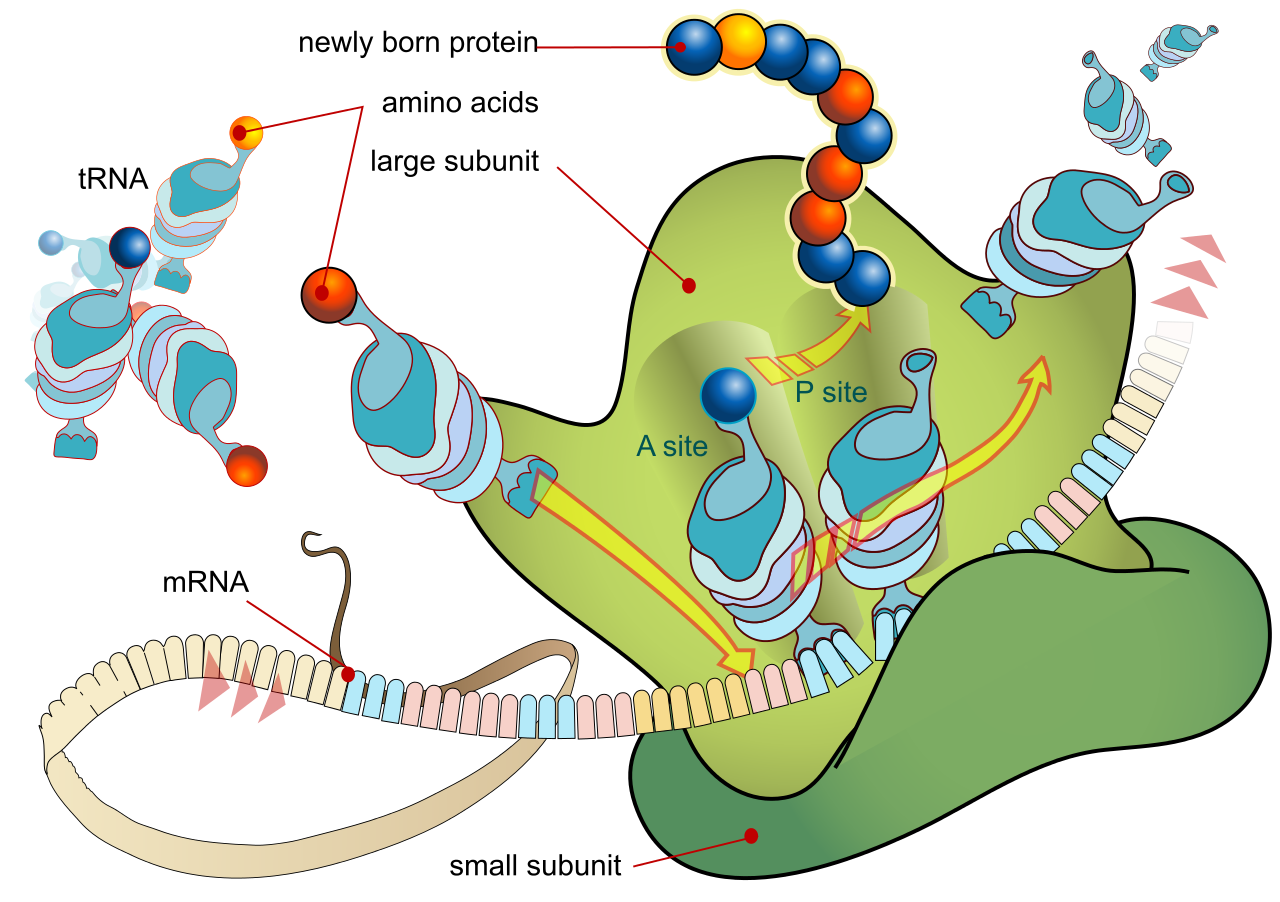
\includegraphics[width=0.99\textwidth]{protein_synthesis}
    \column{0.5\textwidth}
    \centering
    \caption {Finding the global minimum}
    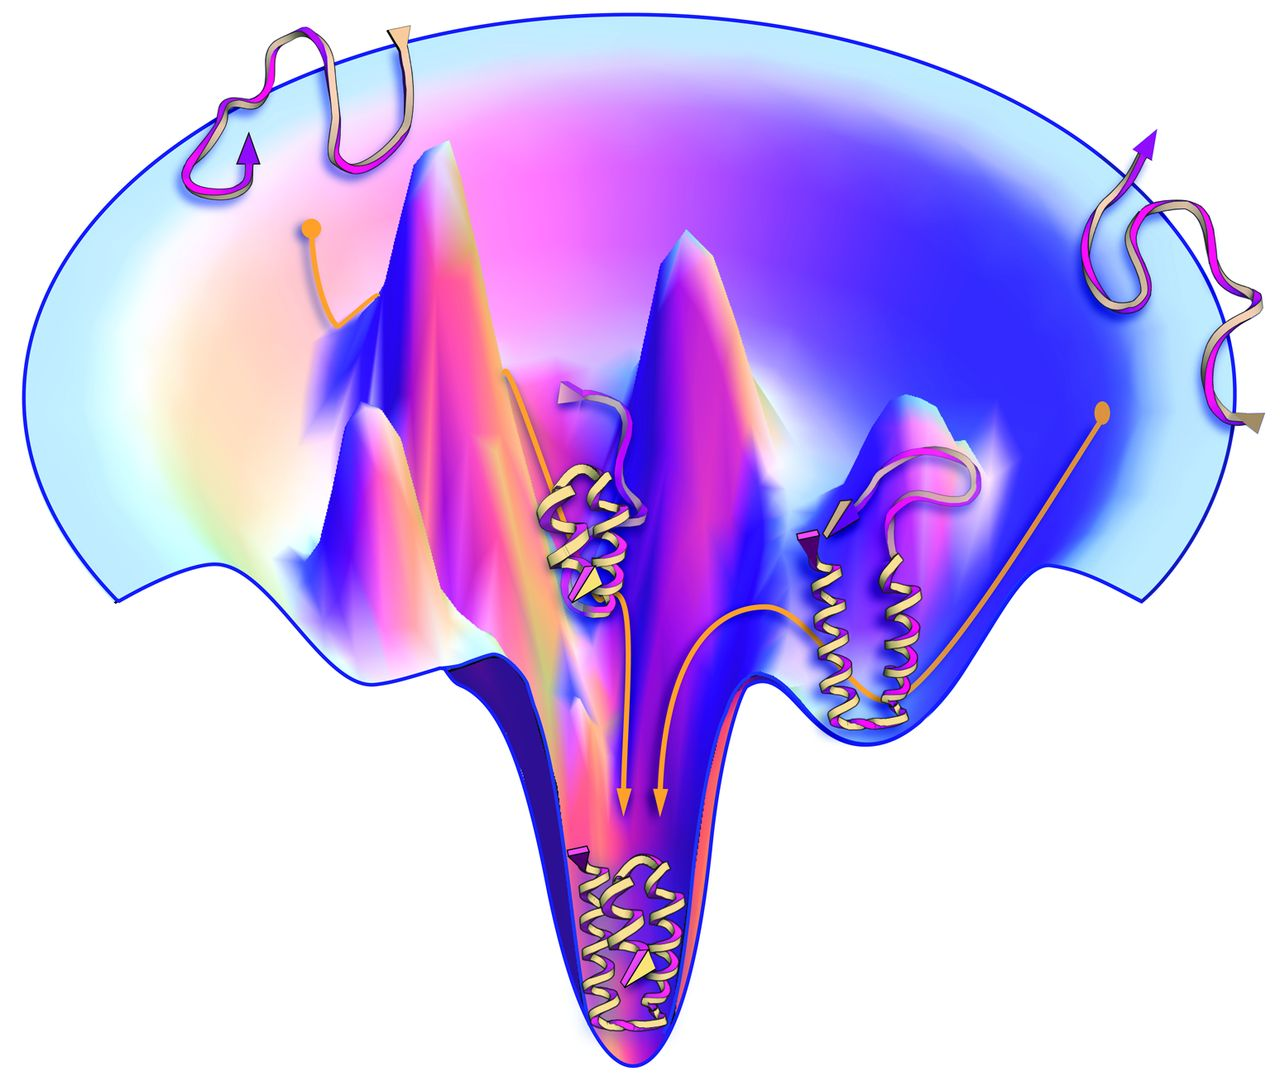
\includegraphics[width=0.99\textwidth]{protein_energy_state}
  \end{columns}
\end{figure}
Folding occurs in microseconds, but cannot be predicted
\end{frame}


\begin{frame}{Abnormal folding}
\begin{figure}
  \centering
  \caption {Deformed proteins cannot be mended}
  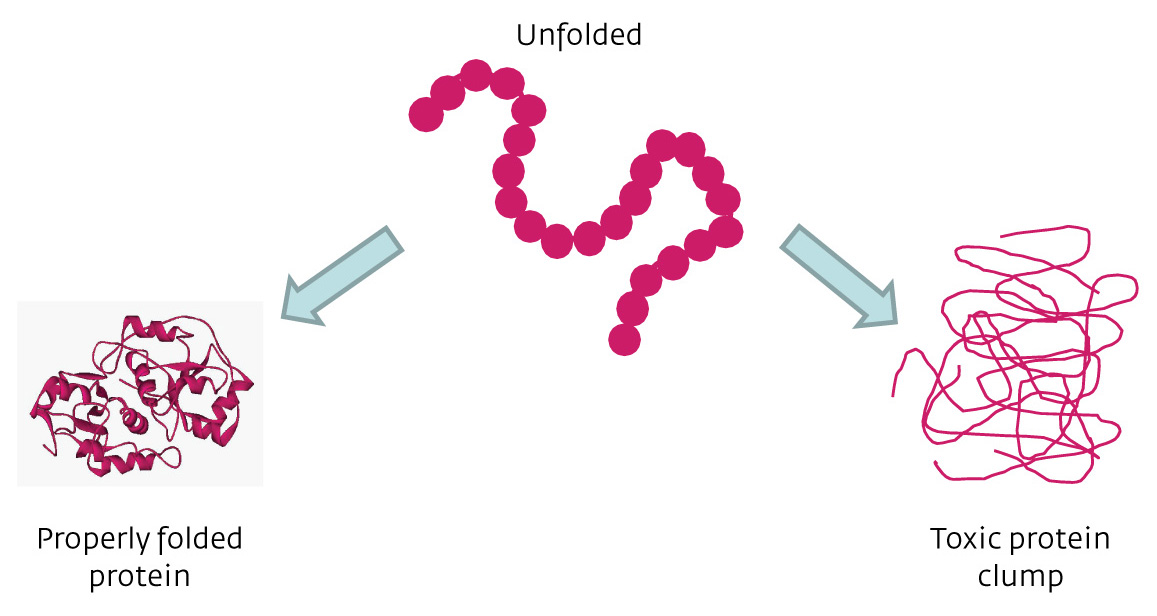
\includegraphics[width=0.7\textwidth]{protein_abnormal_folding}
\end{figure}
\end{frame}


\begin{frame}{In brief}
  \begin{enumerate}
  \item From a chain of amino acids a specific highly complex shape is required\vspace{5mm}
  \item There is no apparent error correction in the process (or very little)\vspace{5mm}
  \item It is usually successful\vspace{5mm}
  \item When it isn't, Creutzfeldt-Jakob disease, Parkinson’s, Alzheimer’s, etc\vspace{5mm}
  \end{enumerate}
\end{frame}


\section{Scientific computation - `\texttt{T = abs(T)}'}


\begin{frame}{Attempts at prediction and projection}
\begin{figure}
  \centering
  \begin{columns}
    \column{0.5\textwidth}
    \centering
    \caption {Numerical approximation}
    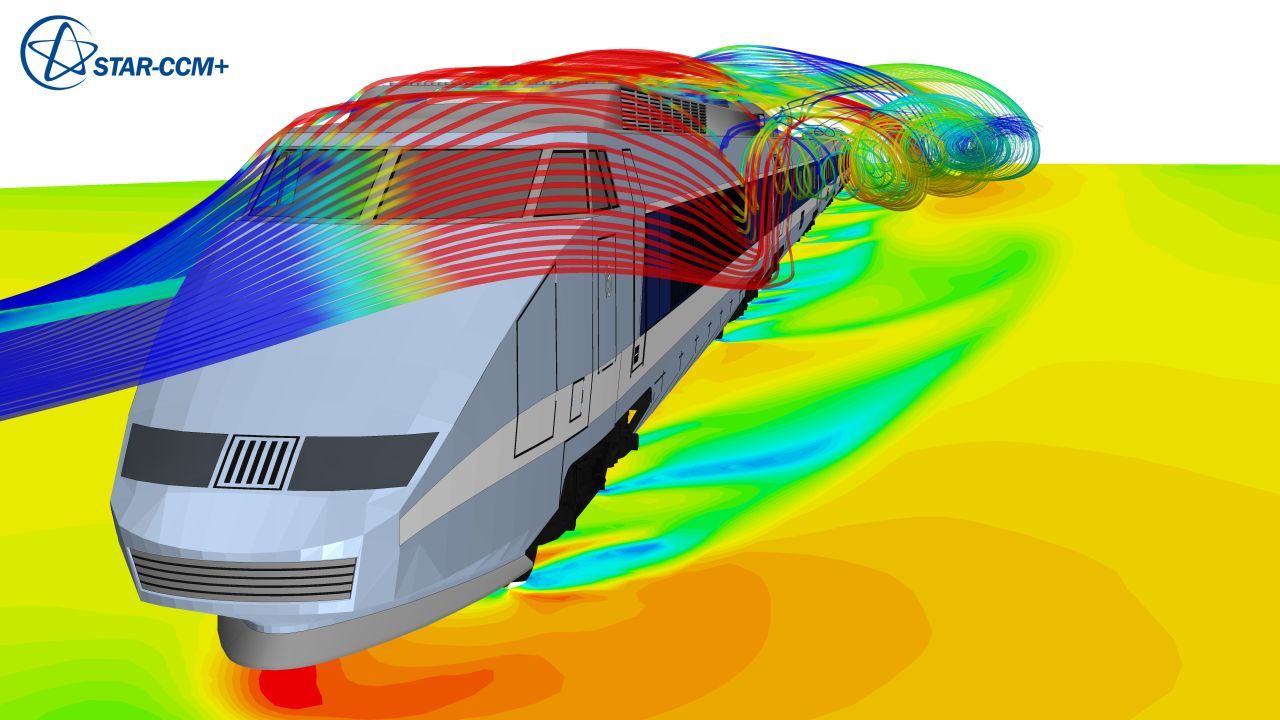
\includegraphics[width=0.99\textwidth]{cfd_train}
    \column{0.5\textwidth}
    \centering
    \caption {Local sensitivities}
    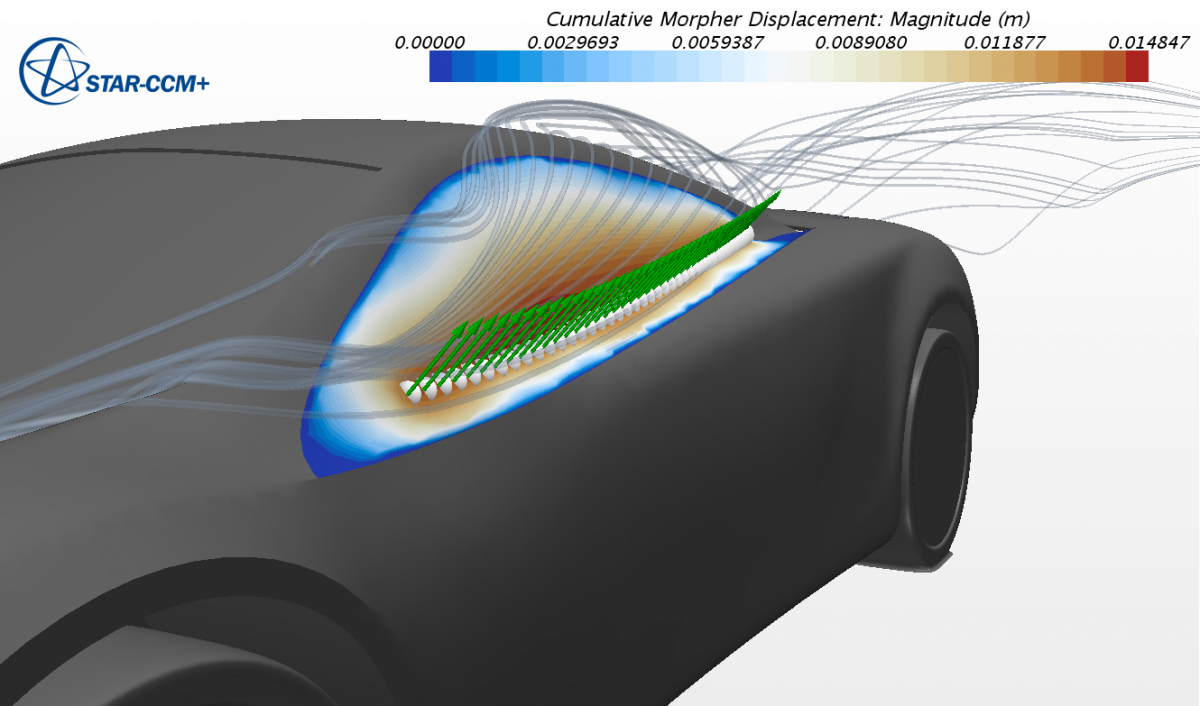
\includegraphics[width=0.99\textwidth]{cfd_car_sensitivity}
  \end{columns}
\end{figure}
Iterative, discretised and linearised algorithms
\end{frame}


\begin{frame}{All starts with a graph (mesh)}
\begin{figure}
  \centering
  \caption {Resolve change at the small scales}
  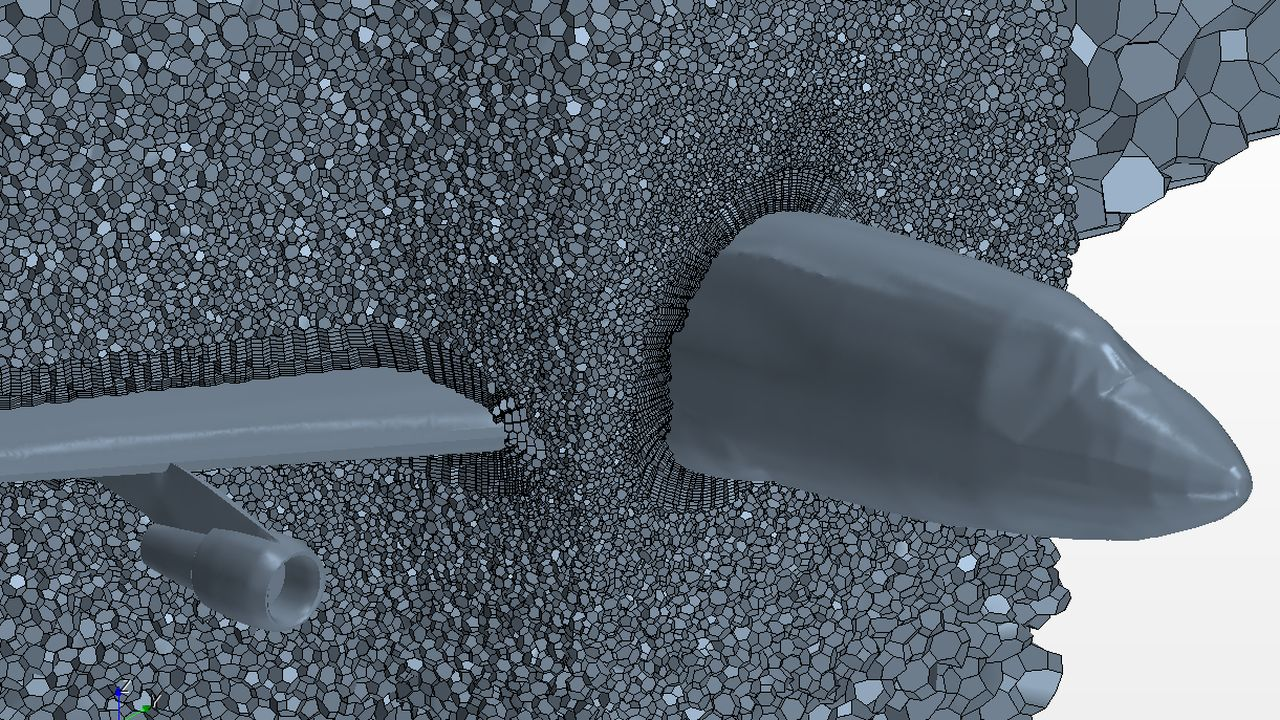
\includegraphics[width=0.7\textwidth]{cfd_mesh_plane}
\end{figure}
Mesh implies graph, implies matrix, implies matrix inversion
\end{frame}


\begin{frame}[fragile]
  \frametitle{Matrix inversion: scaling up}
\begin{lstlisting}[basicstyle=\small\ttfamily]
void inverse(int n, float a[][2*n_max])
{
  for (int i = 0; i < n; i++)
    for (int j = n; j < 2*n; j++)
      a[i][j] = (i == j-n? 1: 0);

  @\aftergroup\redcolor@for@\aftergroup\blackcolor@ (int @\aftergroup\bluecolor@i@\aftergroup\blackcolor@ = 0; i < n; i++) {         // linear
    float aii = a[i][i];
    for (int j = i; j < 2*n; j++)
      a[i][j] = a[i][j] / aii;

    @\aftergroup\redcolor@for@\aftergroup\blackcolor@ (int @\aftergroup\bluecolor@j@\aftergroup\blackcolor@ = 0; j < n; j++) {       // quadratic!
      if (i != j) {
        float aji = a[j][i];
        @\aftergroup\redcolor@for@\aftergroup\blackcolor@ (int @\aftergroup\bluecolor@k@\aftergroup\blackcolor@ = 0; k < 2*n; k++)   // cubic!!
          a[j][k] = a[j][k] - aji * a[i][k]; }}}}
\end{lstlisting}
\end{frame}


\begin{frame}{Computation: slow but compact}
\begin{figure}
  \centering
  \begin{columns}
    \column{0.5\textwidth}
    \centering
    \caption {Geometry and mesh}
    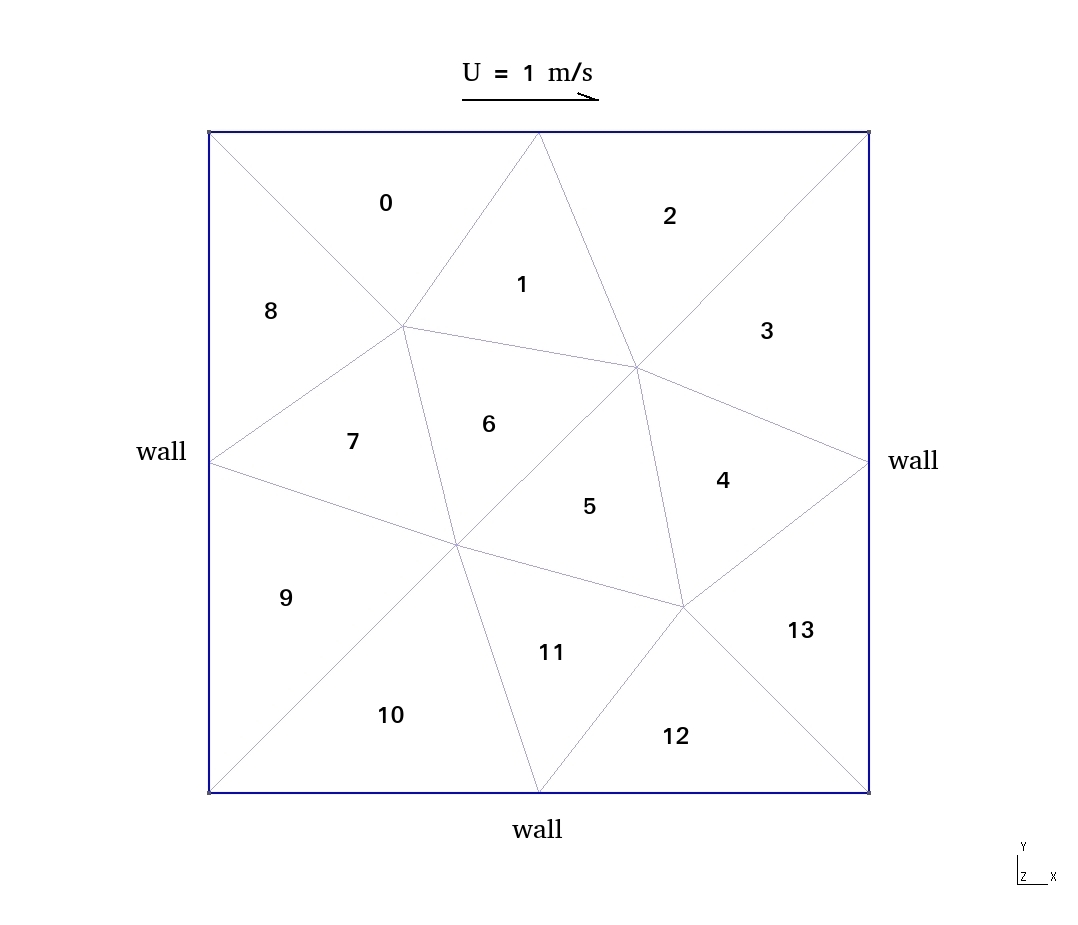
\includegraphics[width=0.99\textwidth]{cavity_2d_tet_i}
    \column{0.5\textwidth}
    \centering
    \caption {Connectivity graph}
    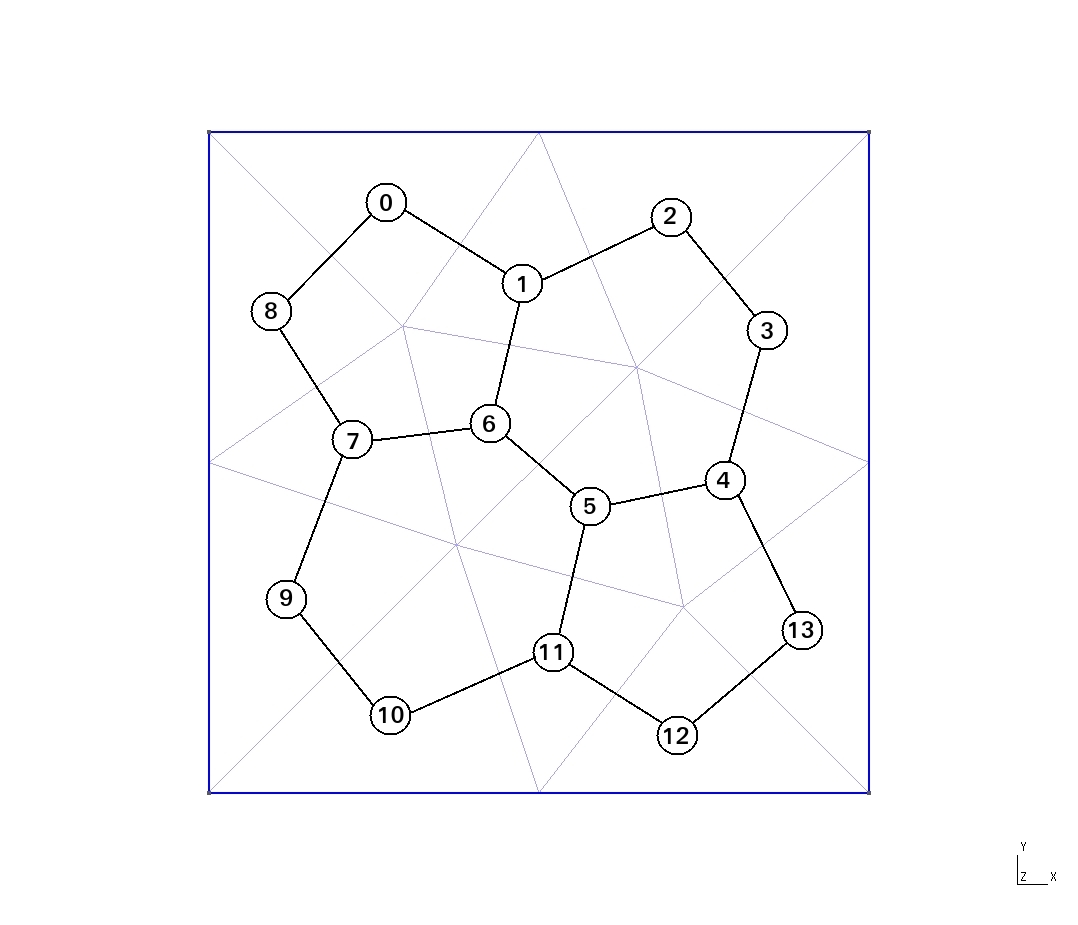
\includegraphics[width=0.99\textwidth]{cavity_2d_tet_d}
  \end{columns}
\end{figure}
\end{frame}


\begin{frame}{Topology Representation}
Symmetric, sparse (48 non-zeros), irregular
  \begingroup
  %% \small
  \tiny
  \centering
\begin{equation*}
\begin{bmatrix}
a_{0,0} & a_{0,1} &  &  &  &  &  &  & a_{0,8} &  &  &  &  & \\
a_{1,0} & a_{1,1} & a_{1,2} &  &  &  & a_{1,6} &  &  &  &  &  &  & \\
& a_{2,1} & a_{2,2} & a_{2,3} &  &  &  &  &  &  &  &  &  & \\
&  & a_{3,2} & a_{3,3} & a_{3,4} &  &  &  &  &  &  &  &  & \\
&  &  & a_{4,3} & a_{4,4} & a_{4,5} &  &  &  &  &  &  &  & a_{4,13} \\
&  &  &  & a_{5,4} & a_{5,5} & a_{5,6} &  &  &  &  & a_{5,11} &  & \\
& a_{6,1} &  &  &  & a_{6,5} & a_{6,6} & a_{6,7} &  &  &  &  &  & \\
&  &  &  &  &  & a_{7,6} & a_{7,7} & a_{7,8} & a_{7,9} &  &  &  & \\
a_{8,0} &  &  &  &  &  &  & a_{8,7} & a_{8,8} &  &  &  &  & \\
&  &  &  &  &  &  & a_{9,7} &  & a_{9,9} & a_{9,10} &  &  & \\
&  &  &  &  &  &  &  &  & a_{10,9} & a_{10,10} & a_{10,11} &  & \\
&  &  &  &  & a_{11,5} &  &  &  &  & a_{11,10} & a_{11,11} & a_{11,12} & \\
&  &  &  &  &  &  &  &  &  &  & a_{12,11} & a_{12,12}  & a_{12,13}\\
&  &  &  & a_{13,4} &  &  &  &  &  &  &  & a_{13,12} &  a_{13,13}
\end{bmatrix}
\end{equation*}
\endgroup
\end{frame}


\begin{frame}[fragile]
  \frametitle{Sparsity and Indirection}
  \begin{itemize}
  \item Dense storage: 196 values, 24\% efficient
  \item Direct access to values
  \end{itemize}
\begin{lstlisting}
  float[14][14] A;
  A[@\aftergroup\redcolor@2@\aftergroup\blackcolor@][@\aftergroup\bluecolor@3@\aftergroup\blackcolor@] = 3.142;
\end{lstlisting}
\vspace{5mm}
  \begin{itemize}
  \item Compressed row storage: 111 values, 56\% efficient
  \item Requires indirection to access values (10x slower)
  \end{itemize}
\begin{lstlisting}
int[15] IA = [0, 3, 7, 10, ...];
int[48] JA = [0, 1, 8,  0, 1, 2, 6,  1, 2, 3,  ...];
float[48] A;

A[JA[IA[@\aftergroup\redcolor@2@\aftergroup\blackcolor@]+2]] = 3.142; // i.e. A[2][3] = 3.142;
\end{lstlisting}
\end{frame}


\begin{frame}{In brief}
  \begin{enumerate}
  \item Many scientific algorithms have graphs and matrices, and perform matrix inversion at their core\vspace{5mm}
  \item They are often woefully inefficient due to the requirement to use compressed storage of irregular data\vspace{5mm}
  \item The compromise on efficiency is to leverage compact memory footprint\vspace{5mm}
  \item In the process of linearising, much of the `beauty' of underlying the mathematics gives way to crude approximation\vspace{5mm}
  \end{enumerate}
\end{frame}


\section{Bridging the Nature --- Computation dichotomy}


\begin{frame}{Artificial Neural Networks}
\begin{figure}
  \centering
  \caption {TensorFlow demo}
  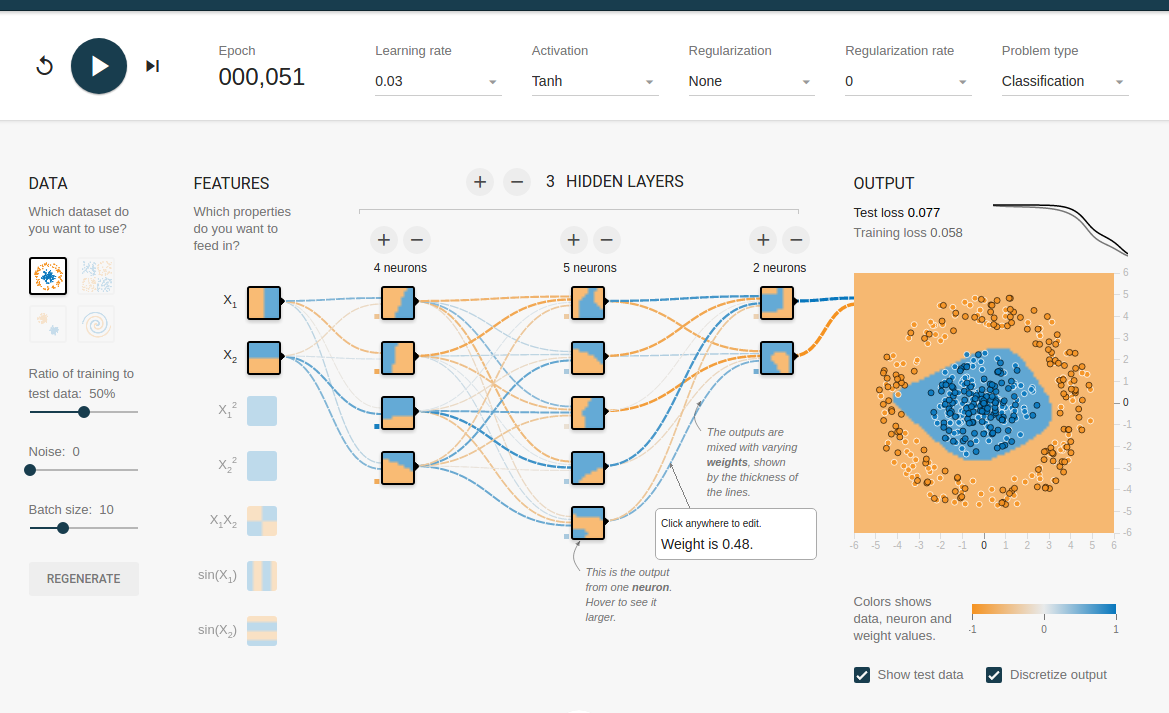
\includegraphics[width=0.9\textwidth]{tensorflow_demo}
\end{figure}
\end{frame}


\begin{frame}{Properties of ANN}
  \begin{enumerate}
  \item Weights are associated with nodes and inter-nodal connections\vspace{5mm}
  \item Processes are relatively straight forward - matrix-vector products and local reductions\vspace{5mm}
  \item Its kernel is essentially plastic - number of hidden layers and number of nodes on each layer govern its form\vspace{5mm}
  \item It has somewhat of the `it should just work' essence - a result will always be produced\vspace{5mm}
  \end{enumerate}
\end{frame}


\begin{frame}{Where the analogy breaks down}
  \begin{enumerate}
  \item \emph{These} nodes and these connections are trained for \emph{this} problem\vspace{5mm}
  \item Training is complicated - requires derivative of every output with respect to every weight\vspace{5mm}
  \item Improvement of the weights requires vast resources relative to evaluating the actual problem\vspace{5mm}
  \end{enumerate}
\end{frame}


\begin{frame}{In brief}
  \begin{enumerate}
  \item Somehow, the need for feedback (or at least how it is presently done) appears to lack a natural analogy\vspace{5mm}
  \item For protein folding, it is as though all possible solutions (and so the right one) are `known' at once\vspace{5mm}
  \item This is somewhat characteristic of quantum computing, and moreover, its solution is \emph{probably} correct\vspace{5mm}
  \end{enumerate}
\end{frame}


\section{Incidentally...}


\begin{frame}{Transpose is like dependency tracing}
  \begin{enumerate}
\item Given a sequence of operations: $\bsym{X}(\bsym{D})$, $\bsym{Q}(\bsym{X})$, $\bsym{L}(\bsym{Q})$,\newline the Jacobian of $\bsym{Q}$ w.r.t. $\bsym{X}$ can be written as
\begin{equation*}
  J_{\bsym{Q}} =
\begin{bmatrix}
  \frac{\partial Q_1}{\partial X_1} & \cdots & \frac{\partial Q_1}{\partial X_n} \\
  \vdots & \ddots & \vdots \\
  \frac{\partial Q_m}{\partial X_1} & \cdots & \frac{\partial Q_m}{\partial X_n}
 \end{bmatrix}
= \frac{\mrm{d} \bsym{Q}}{\mrm{d} \bsym{X}}
\end{equation*}
\item The derivative of the whole system is the chain of the Jacobians of each operation, giving
\begin{equation*}
  \frac{\mrm{d} \bsym{L}}{\mrm{d} \bsym{D}} = \frac{\mrm{d} \bsym{L}}{\mrm{d} \bsym{Q}} \: \frac{\mrm{d} \bsym{Q}}{\mrm{d} \bsym{X}} \: \frac{\mrm{d} \bsym{X}}{\mrm{d} \bsym{D}}
\end{equation*}
  \end{enumerate}
\end{frame}


\begin{frame}{Transpose is like dependency tracing}
  \begin{enumerate}
\item The derivative of the system could be built up by inputting \emph{tangents} of $J_{\bsym{X}}$
\begin{equation*}
  \frac{\mrm{d} \bsym{L}}{\mrm{d} D_{\mrm{i}}} = \frac{\mrm{d} \bsym{L}}{\mrm{d} \bsym{Q}} \: \frac{\mrm{d} \bsym{Q}}{\mrm{d} \bsym{X}} \: \frac{\mrm{d} \bsym{X}}{\mrm{d} D_{\mrm{i}}}
\end{equation*}

\item But by turning the tangents approach ``inside-out'', taking the transpose of the derivative of the system for a particular \emph{gradient} of $J_{\bsym{L}}$
\begin{equation*} \label{eqn:senstivity-transposed}
  \frac{\mrm{d} L_{\mrm{j}}}{\mrm{d} \bsym{D}}^T = \frac{\mrm{d} \bsym{X}}{\mrm{d} \bsym{D}}^T \frac{\mrm{d} \bsym{Q}}{\mrm{d} \bsym{X}}^T \frac{\mrm{d} L_{\mrm{j}}}{\mrm{d} \bsym{Q}}^T
\end{equation*}
offers an efficient way of relating an output to all of its inputs.
  \end{enumerate}
\end{frame}


\begin{frame}[fragile]{Give the output a handle on its history}
  \begin{columns}[T] % align columns
    \begin{column}{.49\textwidth}
        \begin{lstlisting}
auto eval(A const &a,
          B const &b)
{
  auto @\aftergroup\blackcolor@c0@\aftergroup\blackcolor@ = 3;
  auto @\aftergroup\blackcolor@c1@\aftergroup\blackcolor@ = 4;

  auto @\aftergroup\blackcolor@t0@\aftergroup\blackcolor@ = a * b;
  auto t1 = @\aftergroup\blackcolor@c0@\aftergroup\blackcolor@ + @\aftergroup\blackcolor@t0@\aftergroup\blackcolor@;
  auto t2 = @\aftergroup\blackcolor@c1@\aftergroup\blackcolor@ + @\aftergroup\blackcolor@t0@\aftergroup\blackcolor@;
  auto r  = t1 / t2;

  return r;
}
  \end{lstlisting}
    \end{column}%
    \hfill%
    \begin{column}{0.49\textwidth}
\begin{figure}[H]
 \centering
 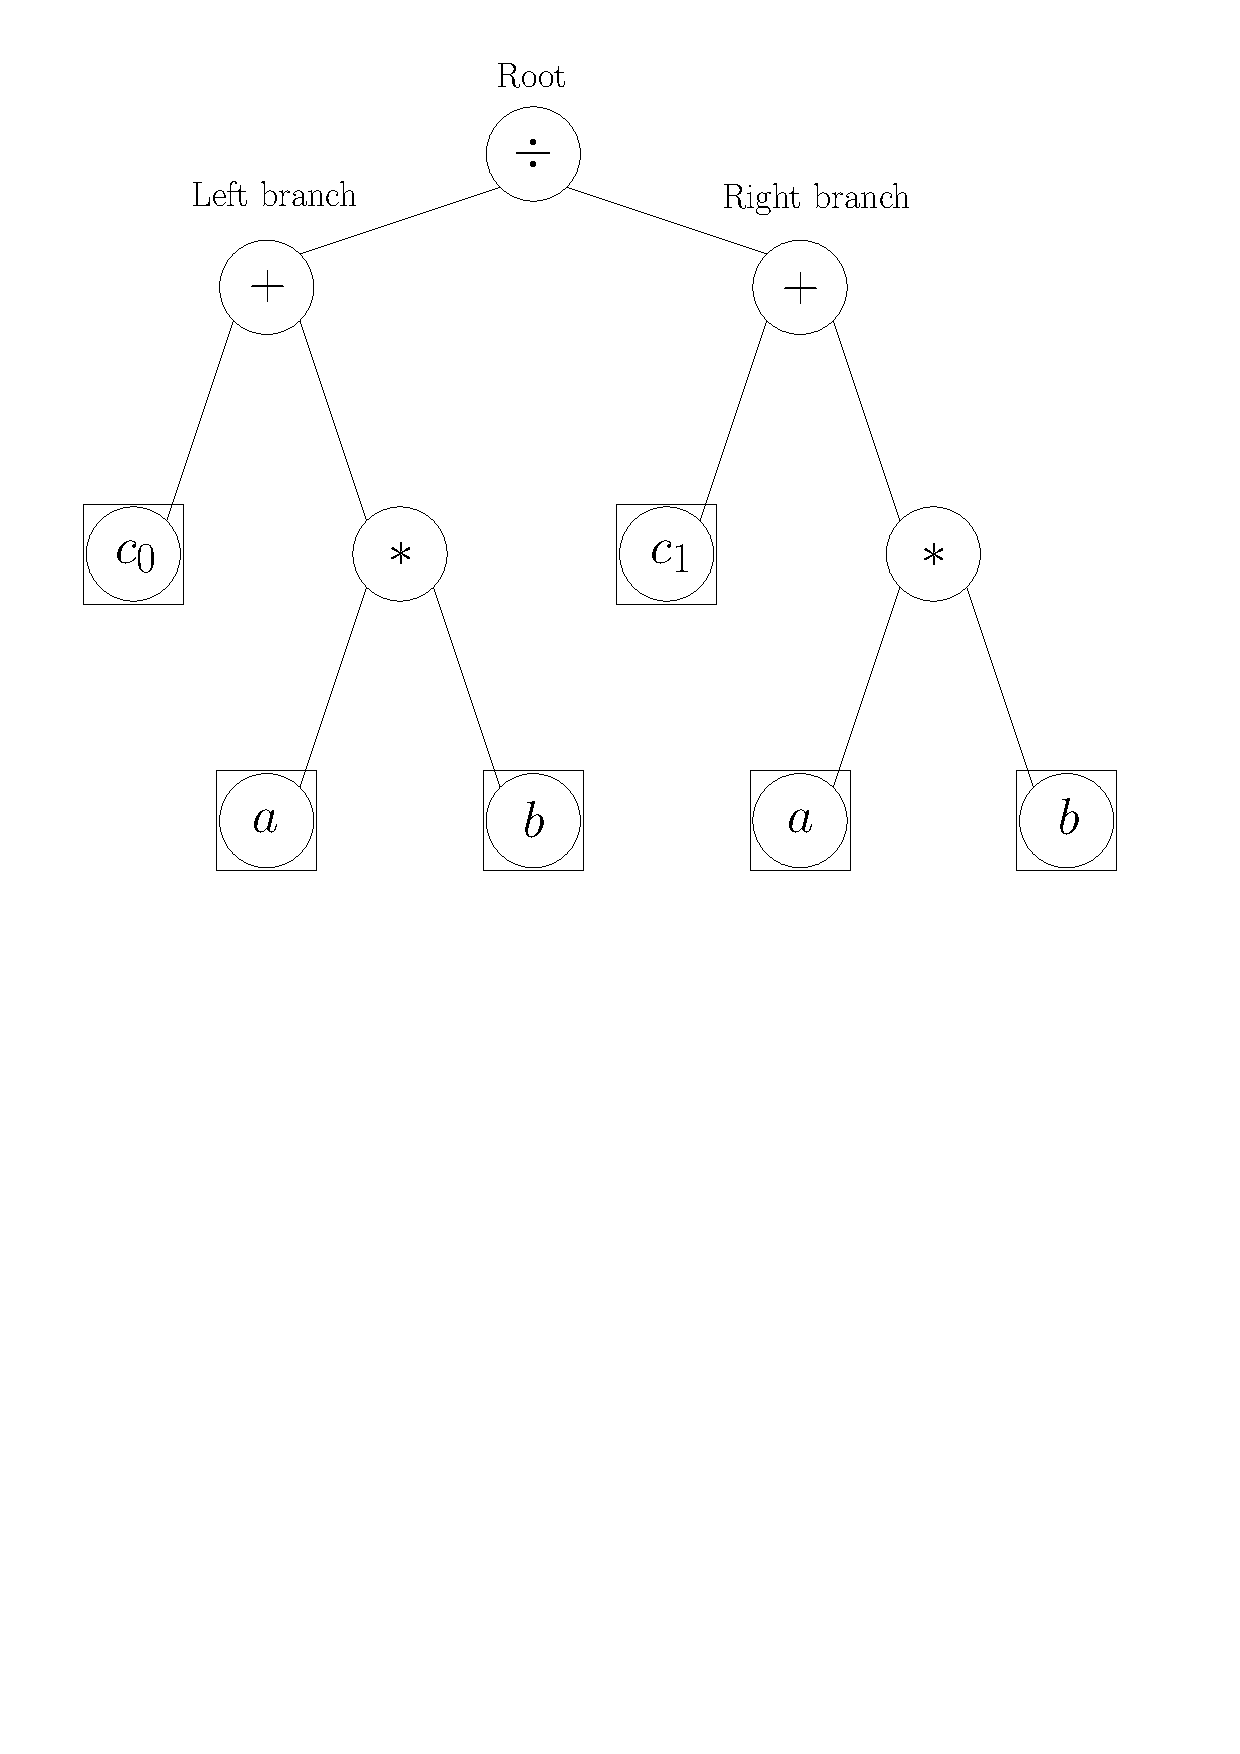
\includegraphics[width=0.99\textwidth]{fig_exprtree}
\end{figure}
    \end{column}%
  \end{columns}
  Instead of computing values, construct expression trees (graphs!)
\end{frame}


\begin{frame}[fragile]{`Adjoint' differentiation}
  Apply the chain rule and transpose...
  \begin{columns}[T] % align columns
    \begin{column}{.49\textwidth}
      \begin{lstlisting}
  t0 = a * b     // 1
  t1 = c0 + t0   // 2
  t2 = c1 + t0   // 3
  r  = t1 / t2   // 4
  \end{lstlisting}
    \end{column}%
    \hfill%
    \begin{column}{0.49\textwidth}
        \begin{lstlisting}



  // 4
  t1_d += (1 / t2)    * r_d
  t2_d -= (t1 / t2^2) * r_d

  // 3
  t0_d += t2_d

  // 2
  t0_d += t1_d

  // 1
  a_d  += b * t0_d
  b_d  += a * t0_d
  \end{lstlisting}
    \end{column}%
  \end{columns}
\end{frame}


\begin{frame}{Directed design}
\begin{figure}
  \centering
  \caption {Move surface {\redcolor{in}} or {\bluecolor{out}} to reduce drag}
  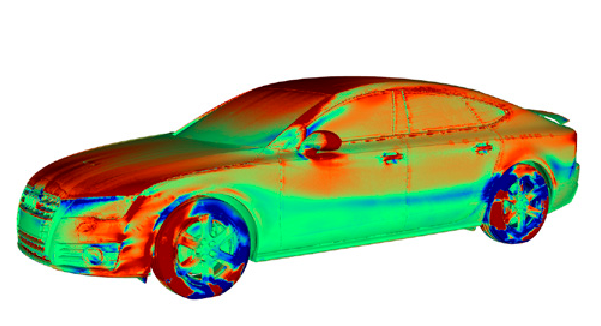
\includegraphics[width=0.9\textwidth]{cfd_audi_sensitivity}
\end{figure}
\end{frame}


\begin{frame}{In brief}
  \begin{enumerate}
  \item There is some analogy with entanglement and wave function collapsing in classical computation\vspace{5mm}
  \item It gives all solutions in one evaluation\vspace{5mm}
  \item But, everything really is back-to-front! (and implementing it is a nightmare!)\vspace{5mm}
  \end{enumerate}
\end{frame}


\end{document}


%% \begin{frame}[fragile]
%%   \frametitle{Intersection of two lines}
%% \begin{figure}
%%   \centering
%%   \begin{columns}
%%     \column{0.5\textwidth}
%%     \centering
%%   \begin{eqnarray*}
%%     -0.35x + y &=& 2\\
%%     2.5x - 2y &=& 4
%%   \end{eqnarray*}
%%   \begin{eqnarray*}
%%     \begin{bmatrix}
%%       -0.35 & 1 \\
%%       2.5 & -2
%%     \end{bmatrix}
%%     \begin{bmatrix}
%%       x \\
%%       y
%%     \end{bmatrix}
%%     &=&
%%     \begin{bmatrix}
%%       2 \\
%%       4
%%     \end{bmatrix}
%%   \end{eqnarray*}
%%   %% \begin{eqnarray*}
%%   %%   A x = b
%%   %% \end{eqnarray*}
%%   \begin{eqnarray*}
%%     \begin{bmatrix}
%%       x \\
%%       y
%%     \end{bmatrix}
%%     &=&
%%     \begin{bmatrix}
%%       -0.35 & 1 \\
%%       2.5 & -2
%%     \end{bmatrix}^{-1}
%%     \begin{bmatrix}
%%       2 \\
%%       4
%%     \end{bmatrix}
%%   \end{eqnarray*}
%%   %% \begin{eqnarray*}
%%   %%   x = A^{-1} b
%%   %% \end{eqnarray*}
%%   Matrix inverse?
%%   \column{0.5\textwidth}
%%     \centering
%%     %% \caption {Plot of intersecting lines}
%%     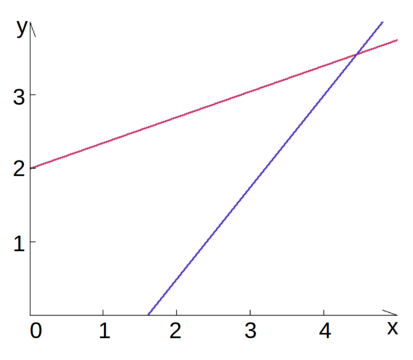
\includegraphics[width=0.9\textwidth]{intersecting_lines}
%%   \end{columns}
%% \end{figure}
%% \end{frame}


%% \begin{frame}[fragile]
%%   \frametitle{Division (scalar inverse)}
%%   \begin{lstlisting}[basicstyle=\tiny\ttfamily]
%% unsigned divide(unsigned a, unsigned b)
%% {
%%   unsigned denom = b, current = 1, result = 0;

%%   if (denom > a) return 0;
%%   if (denom == a) return 1;

%%   while (denom <= a) {
%%     denom <<= 1;
%%     current <<= 1;
%%   }

%%   denom >>= 1;
%%   current >>= 1;

%%   @\aftergroup\redcolor@while@\aftergroup\blackcolor@ (current != 0) {  // n^1
%%     if (a >= denom) {
%%       a -= denom;
%%       result |= current;
%%     }

%%     current >>= 1;
%%     denom >>= 1;
%%   }

%%   return result;
%% }
%% \end{lstlisting}
%% \end{frame}


%% \begin{frame}{Accuracy}
%% \begin{figure}
%%   \centering
%%   \begin{columns}
%%     \column{0.5\textwidth}
%%     \centering
%%     \caption {Coarse mesh (48 elements)}
%%     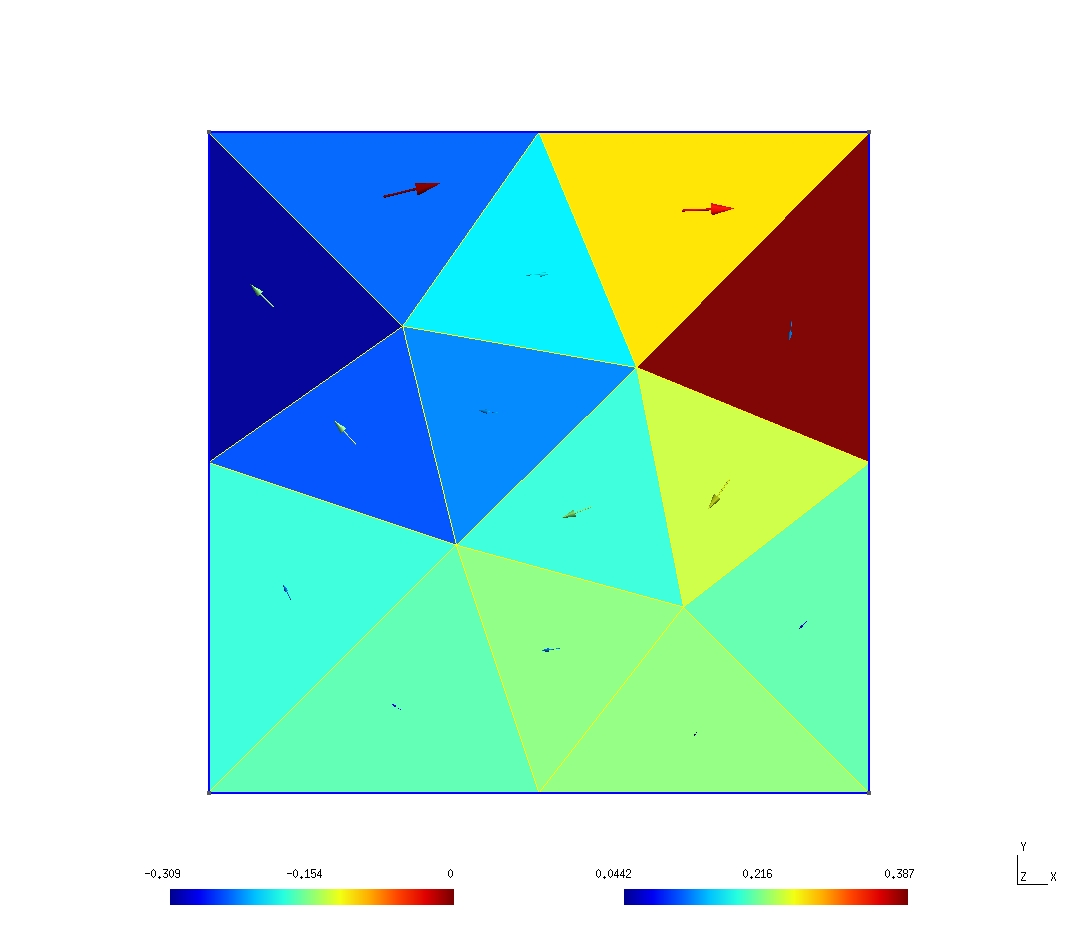
\includegraphics[width=0.99\textwidth]{cavity_2d_tet_coarse}
%%     \column{0.5\textwidth}
%%     \centering
%%     \caption {Fine mesh (132,607 elements)}
%%     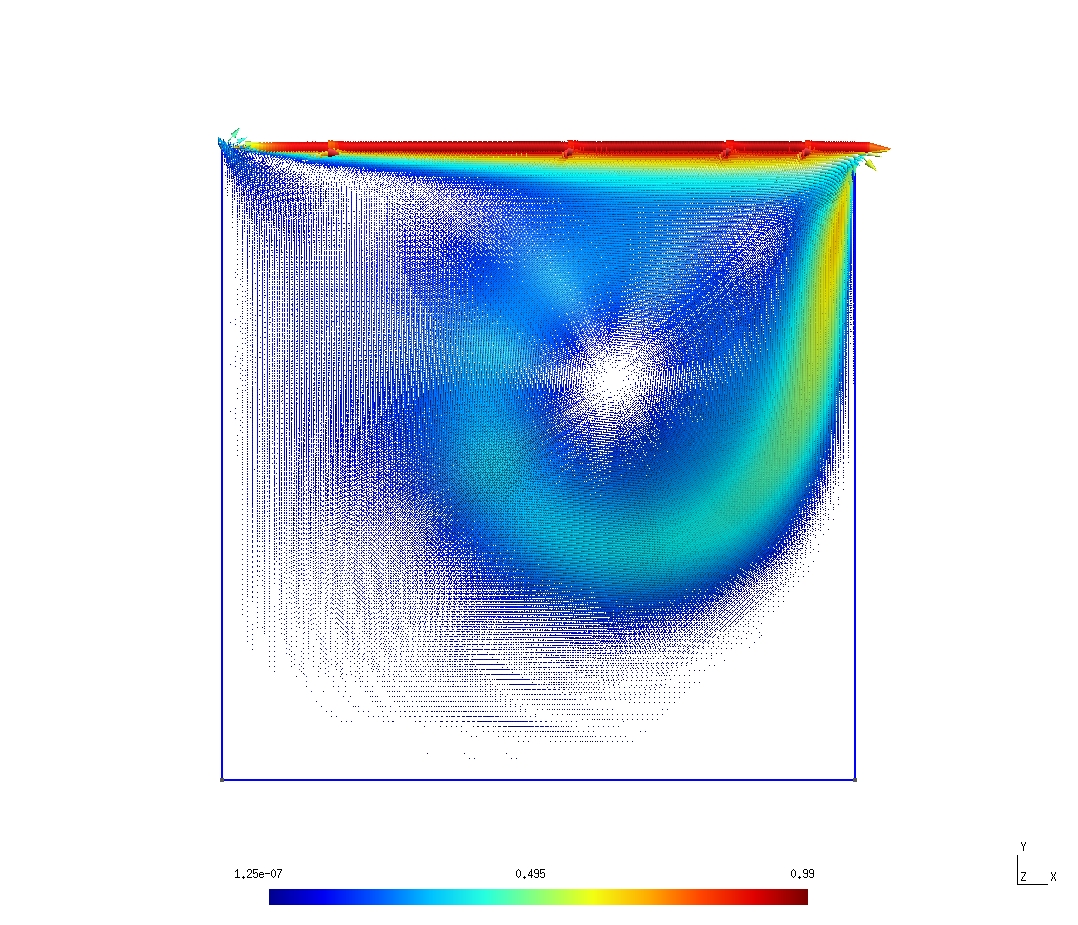
\includegraphics[width=0.99\textwidth]{cavity_2d_tet_fine}
%%   \end{columns}
%% \end{figure}
%% \end{frame}


%% \begin{frame}{Speed}
%%   \begin{enumerate}
%%   \item Partition the mesh into four chunks
%%   \item Each CPU core computes one chunk
%%   \item Communication eventually swamps computation
%%   \end{enumerate}
%% \begin{figure}
%%   \centering
%%   \begin{columns}
%%     \column{0.5\textwidth}
%%     \centering
%%     %% \caption {Cavity flow}
%%     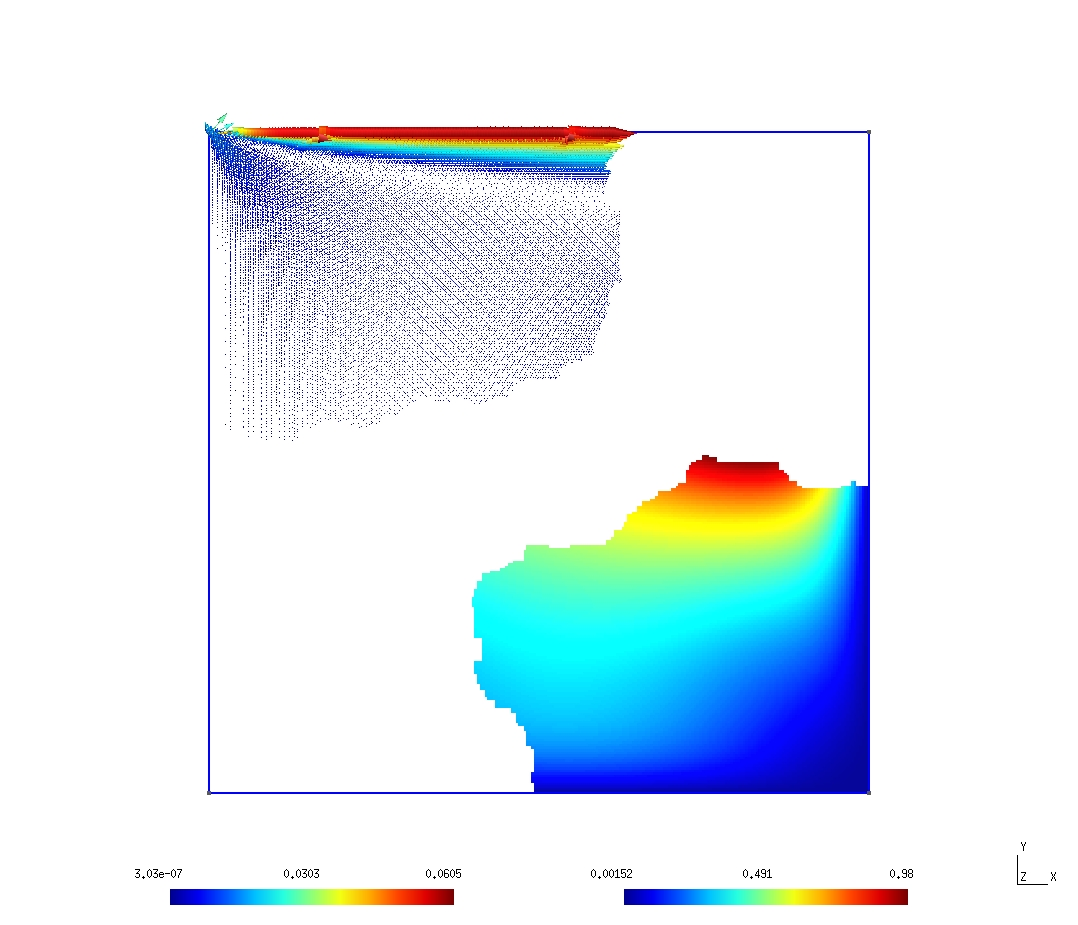
\includegraphics[width=0.99\textwidth]{cavity_2dp_tet_fine}
%%     \column{0.5\textwidth}
%%     \centering
%%     %% \caption {Duct flow}
%%     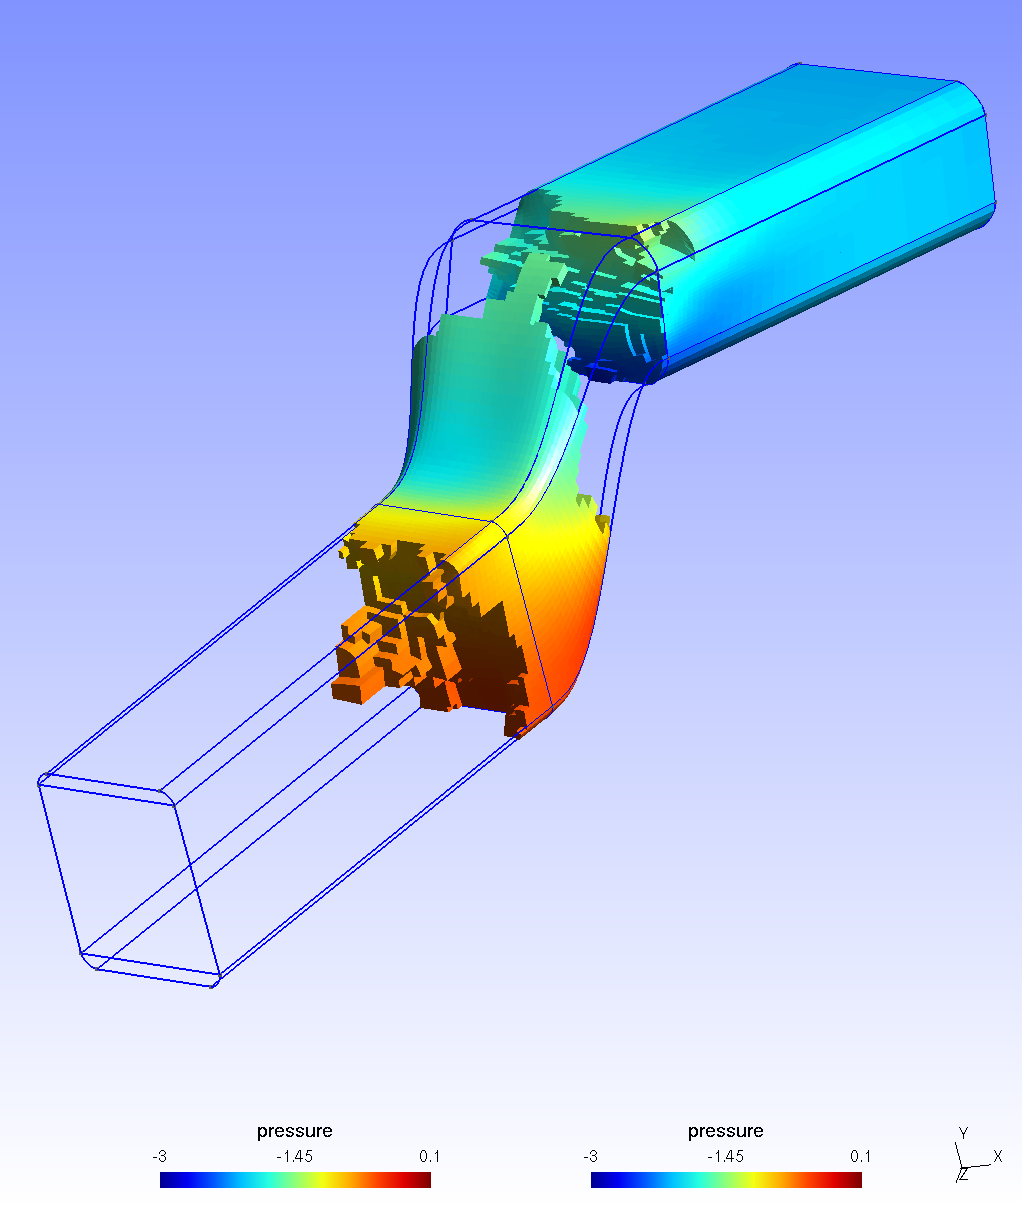
\includegraphics[width=0.85\textwidth]{duct_3d_4p}
%%   \end{columns}
%% \end{figure}
%% \end{frame}
